\documentclass[11pt,a4paper]{article}
\usepackage[utf8]{inputenc}
\usepackage[T1]{fontenc}
\usepackage[english]{babel}
\usepackage[margin=2.1cm]{geometry}
\usepackage{booktabs,array,tabularx}
\usepackage{xcolor}
\usepackage{graphicx}
\usepackage{pgfplots}
\pgfplotsset{compat=1.17}
\PassOptionsToPackage{hyphens}{url}
\usepackage[hidelinks]{hyperref}
\usepackage{enumitem}
\setlist{nosep,leftmargin=1.4em}
\emergencystretch=3em

\definecolor{impl}{HTML}{3B6EA8}
\definecolor{rev}{HTML}{8FB3DA}

\title{Sweatshop on P-Chess: three tickets from Bruno's QA\\\large Held piece survives Maia's reply (UI-011), human reaction time for Maia (BOT-009) and a whole-second clock calibration (BOT-010); GPT-6.1 Sol lineup, lane \texttt{qa}}
\author{Foreman, session \texttt{sweatshop/qa/2026-10-27-1653}}
\date{27 October 2026}

\begin{document}
\maketitle

\section*{Summary}

A lane run (\texttt{-Lane qa}) in a fresh clone at \path{.artifacts-build/lanes/qa}, default
lineup \texttt{sol}. All three tickets are \texttt{Difficulty: hard}, so stage 2 ran on the
lineup's hard model, \texttt{gpt-6.1-sol xhigh}, the same model as the reviewer. Before launch
the clone's gate passed (258 passed, 0 failed) and the ignored Lc0 binary and Maia nets were
copied in from the main checkout. Launch at 16:53, ``Nothing runnable'' at 17:44.
UI-009 (blocked on sound research in another session) and CI-003 (blocked on Bruno's clean-Windows
game) were out of scope and untouched.

\begin{itemize}
  \item \textbf{Produced:} UI-011, BOT-009 and BOT-010 merged on the session at the first
        attempt, \texttt{Verdict: Approve}, 0 findings each. BOT-010 is \texttt{Review: human}.
        Session PR \href{https://github.com/Laginho/P-Chess/pull/22}{\#22}; gate 268 passed,
        0 failed (258 on \texttt{main} before the run); Python calibration tests 14 passed.
  \item \textbf{Cost:} \textbf{\$5.86} at API list price over 6 stages, all
        \texttt{gpt-6.1-sol xhigh}: \$3.55 stage 2, \$2.30 review. Codex quota: 2 points of the
        weekly window (stage 2 1, review 1, each $\pm$1).
  \item \textbf{What went wrong:} nothing in the run. Every ticket still owes a manual game
        (product acceptance pending).
  \item \textbf{Provisional verdict:} clean and fast (17~min per ticket end to end, \$1.95 per
        ticket). Hard tickets on \texttt{xhigh} cost about twice the \texttt{high} stage 2 of
        25 October.
\end{itemize}

\section*{What was done}

\textbf{UI-011}: when you hold a piece (dragging or click-selected) while Maia thinks and Maia
moves, the hold now continues and the drop counts against the new position, as on Lichess and
Chess.com. If Maia captured or moved the held piece, the hold ends; legal-move dots refresh; an
open promotion picker still closes. Main file \path{ui/board_view.gd} (\texttt{\_commit}).

\textbf{BOT-009}: Maia no longer answers instantly to a hung piece. An ordinary move now waits at
least 0.4~s (\texttt{REACTION}, an initial value to tune by playing), so Maia's clock can reach
zero in a 1+0 scramble. The 0.05~s ``premove'' floor now needs the human's last move to have
been Maia's top prediction, top\_p over 0.9 and under 10\% of the starting time; Maia asks
Lc0 for that prediction with one extra policy query. Main files \path{bot/time_model.gd} and
\path{bot/maia_player.gd}.

\textbf{BOT-010}: the think-time table is recalibrated. The script now fits the log-normal to
Lichess's whole-second clocks (interval-censored likelihood) and samples up to 1,000 positions
per (control, level, clock bin), so the 1+0 scramble buckets have data: 243 buckets, 216--479
samples in each of the 27 scramble buckets, from a 20~MB prefix of the September 2026 dump.
Main files \path{scripts/calibrate_time.py} and \path{data/time_model.json}.

\section*{Timeline}

\begin{tabularx}{\linewidth}{@{}lX@{}}
\toprule
16:51 & Clone of \texttt{origin} at \texttt{bc36ac9}; gate 258/0; engine files copied. \\
16:53 & Launch, pid 29500; session \texttt{sweatshop/qa/2026-10-27-1653}. UI-011 stage 2. \\
17:05 & UI-011 to review. \\
17:08 & UI-011 merged, 0 findings. BOT-009 stage 2. \\
17:19 & BOT-009 to review. \\
17:22 & BOT-009 merged, 0 findings. BOT-010 stage 2. \\
17:32 & BOT-010: two proxy decisions (GPT-6 Astra fallback) on the download size. \\
17:39 & BOT-010 to review. \\
17:44 & BOT-010 merged, 0 findings; ``Nothing runnable''; PR \#22 opened. \\
\bottomrule
\end{tabularx}

\section*{Per stage}

{\small
\begin{tabularx}{\linewidth}{@{}llllrrrrrX@{}}
\toprule
When & Ticket & Stage & Model & Min & In & Cache & Out & Cost & Outcome \\
\midrule
17:05 & UI-011 & impl & sol xhigh & 12 & 3.1M & 97\% & 22k & 1.01 & to-review \\
17:08 & UI-011 & review & sol xhigh & 3 & 1.7M & 89\% & 9k & 0.75 & merged \\
17:19 & BOT-009 & impl & sol xhigh & 11 & 3.1M & 97\% & 25k & 1.03 & to-review \\
17:22 & BOT-009 & review & sol xhigh & 3 & 2.1M & 93\% & 10k & 0.79 & merged \\
17:39 & BOT-010 & impl & sol xhigh & 17 & 5.2M & 98\% & 28k & 1.51 & to-review \\
17:44 & BOT-010 & review & sol xhigh & 4 & 2.1M & 94\% & 12k & 0.76 & merged \\
\midrule
 & & & & 50 & 17.3M & & 106k & 5.86 & \\
\bottomrule
\end{tabularx}
}

\begin{center}
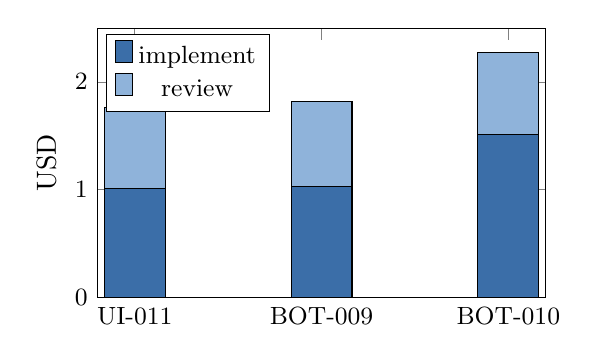
\begin{tikzpicture}
\begin{axis}[ybar stacked, bar width=22pt, width=0.6\linewidth, height=5cm,
  symbolic x coords={UI-011,BOT-009,BOT-010},
  xtick=data, ylabel={USD}, ymin=0, legend style={at={(0.02,0.98)},anchor=north west,font=\small},
  tick label style={font=\small}]
\addplot[fill=impl] coordinates {(UI-011,1.01) (BOT-009,1.03) (BOT-010,1.51)};
\addplot[fill=rev] coordinates {(UI-011,0.75) (BOT-009,0.79) (BOT-010,0.76)};
\legend{implement, review}
\end{axis}
\end{tikzpicture}
\end{center}

Wasted: none in the driver. Inside BOT-010's stage 2, a first calibration attempt with a 500~MB
cap was stopped before producing a table (parsing projected about two hours); its download is
estimated at 200~MB, within Bruno's 500~MB approval.

\section*{Comparison with previous runs}

From \texttt{run-log.md}: the 25 October \texttt{sol} run cost \$4.18 for three tickets with stage
2 on \texttt{gpt-6.1-sol high} (\$0.43--0.98 per stage 2). This run's stage 2 on \texttt{xhigh}
cost \$1.01--1.51, for hard tickets; reviews cost the same (\$0.57--0.91 then, \$0.75--0.79 now).
BOT-010 is the most expensive ticket (\$2.27): stage 2 ran a real calibration over Lichess data.

\section*{Observations per model}

\begin{itemize}
  \item \textbf{gpt-6.1-sol xhigh, stage 2}: three handoffs at the first attempt, 11--17~min,
        each with red test commits before the fix and a final red replay against the old
        production file. UI-011 changed one existing test's expectation, as its ticket asked.
        BOT-009 edited three existing test files only to feed the new prediction reply (no
        assertion weakened). BOT-010 loosened one CLI assertion (exact median $\to$ between 2
        and 4~s) because the rounded-clock fit no longer equals the raw median; the per-stratum
        bound is tested by a separate test.
  \item \textbf{gpt-6.1-sol xhigh, review}: three reviews, 3--4~min, 0 findings, no code in
        review (no round-0 rows), all reusing the stage-2 gate receipt. The BOT-010 review noted
        and accepted missing commit bodies as a Standards exception.
\end{itemize}

\section*{Driver and runtime issues}

\begin{enumerate}
  \item None in the driver: no crash, retry or restart; shutdown 1.3--1.8~s per stage.
  \item \path{.artifacts-build/} was not ignored in the main checkout; the foreman added it to
        \texttt{.git/info/exclude}, and the clone's exclude got the run-log paths (excludes are
        not cloned).
  \item A fresh clone lacks the ignored \path{engine/lc0} and \path{engine/weights}; without
        them four Lc0 tests skip. The foreman copied them from the main checkout.
\end{enumerate}

\section*{Recommendations}

\begin{enumerate}
  \item Play the three manual checks below before tagging a release; BOT-009's 0.4~s and
        BOT-010's table are tuned by feel, not by tests.
  \item Lane clones: document the engine copy as a clone setup step next to the excludes.
  \item Keep \texttt{gpt-6.1-sol xhigh} for hard tickets: scoreboard row
        \texttt{gpt-6.1-sol xhigh} $\rightarrow$ \texttt{gpt-6.1-sol xhigh}, 9 reviews, 1
        reopened (11\%), S2 rate 11\% --- under 10 reviews, an anecdote.
\end{enumerate}

\section*{Human debt and proxy decisions}

No \texttt{Débito humano:} lines. Proxy decisions of this run, both on BOT-010 by the
GPT-6 Astra fallback:

\begin{itemize}
  \item ``start with a 20 MB compressed prefix and increase only if coverage is insufficient,
        within the cumulative 500 MB download budget; acceptance still requires all 27 real
        1+0/clock\_bin 0 buckets with at least 50 samples each.''
  \item ``reserve an estimated 200 MB for the interrupted attempt and proceed with the 20 MB
        prefix. Including the earlier 20 MB probe, conservative accounting reserves 240 MB of
        500 MB and leaves 260 MB.''
\end{itemize}

\section*{Reopen attribution}

No reopened review and no fix made in review in this run, so no new rows in
\path{reopen-attribution.md}. No session-review, release-audit or post-release finding was
reported since the last pass (the Copilot reviewer on PR \#22 did not run, out of quota).

\section*{Scoreboard}

\texttt{scoreboard.ps1} over the ClassyCall, EasyMath, P-Chess, PhysiSyst, SIGAA-ME and
SynchroNice main checkouts (no lane clone). Moved since the 25 October report:
\texttt{gpt-6.1-sol xhigh} $\rightarrow$ \texttt{gpt-6.1-sol xhigh} from 6 to 9 reviews, still
1 reopened (17\% $\to$ 11\%), an anecdote. \texttt{gpt-6.1-sol high} $\rightarrow$
\texttt{gpt-6.1-sol xhigh} unchanged at 18 reviews, 22\%. The implementer row
\texttt{gpt-6.1-sol xhigh}: 9 stage runs, 9 to review, 0 failed, median 12~min. Interventions
printed before this run's two proxy rows were committed: human-rescue 24, routine-approval 18,
proxy-decision (gpt-6-astra high, fallback) 44, (opus) 33.

\section*{Pending for the human}

\begin{enumerate}
  \item UI-011: a 1+0 game; start dragging before Maia replies and drop after; the move plays.
  \item BOT-009: a 1+0 game; hang a piece with Maia under 6~s (it does not move instantly);
        a premove-only scramble where Maia's clock reaches zero. Tune \texttt{REACTION} if needed.
  \item BOT-010 (\texttt{Review: human}): a few 1+0 and 5+0 games against the new table;
        judge the think-time spread.
  \item Review and merge session PR \#22.
\end{enumerate}

\end{document}
